Esta captura se realizó a partir de una red doméstica, con dos computadoras conectadas por cable ethernet y varios dispositivos wireless (laptops, celulares, impresora y chromecast).

\textbf{Fuente S}:

La entropía obtenida (aproximadamente 0.924) se acerca bastante a la máxima, a diferencia de las otras capturas que poseen una entropía muy baja. Además como se observa en el gráfico, la proporción de mensajes unicast fue mayor que la de broadcast.	

\begin{figure}[H]
\centering
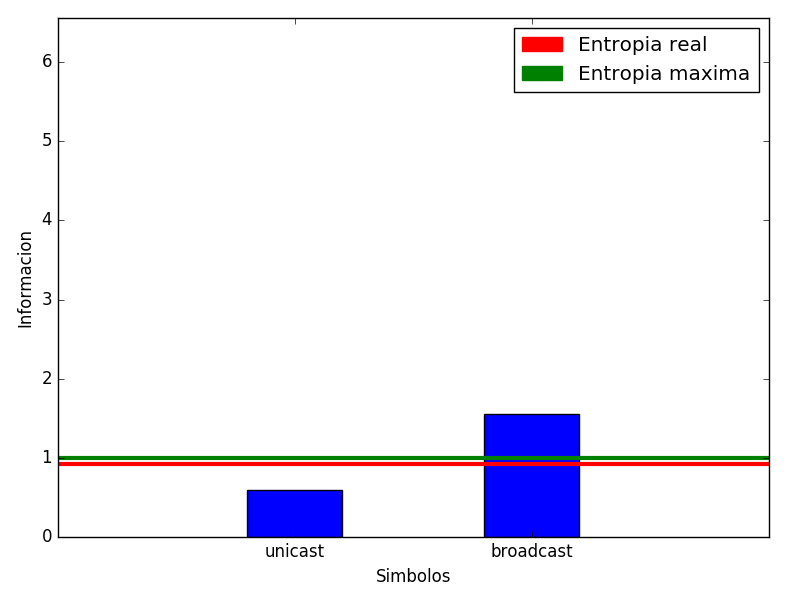
\includegraphics[keepaspectratio=true,scale=1,width=1\linewidth]{imagenes/red-dom-S}
\caption{Red doméstica - Fuente S}
\label{fig:red-dom-S}
\end{figure}

Todo este comportamiento se debe a que al haber pocos dispositivos dentro de la red y tratándose siempre de los mismos, las tablas ARP de cada nodo se mantienen más estables (menos probabilidad de anomalías) y los mensajes broadcast se observan con menos frecuencia.

\textbf{Fuente S1}:

El análisis a partir de S1 (no se agruparon nodos por tratarse de una red pequeña), muestra un único nodo distinguido que coincide con el default gateway de la red (192.168.0.1).

\begin{figure}[H]
	\centering
	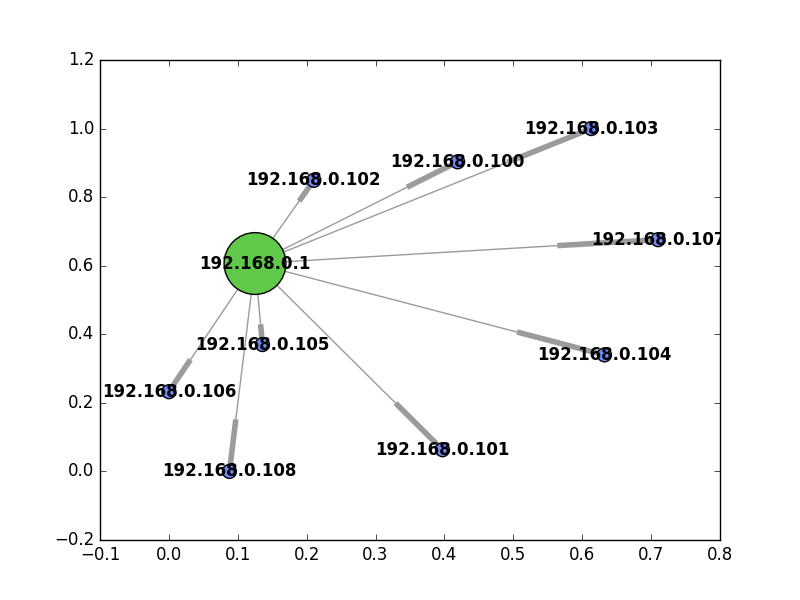
\includegraphics[width=0.8\linewidth]{imagenes/grafo-red-luis.png}
	\caption{Grafo derivado de S1 }
	\label{fig:eth-red-domestica}
\end{figure}

Para tener un análisis más detallado generamos el grafo con las mismas condiciones que antes pero agregando las conexiones entre nodos no distinguidos.

\begin{figure}[H]
	\centering
	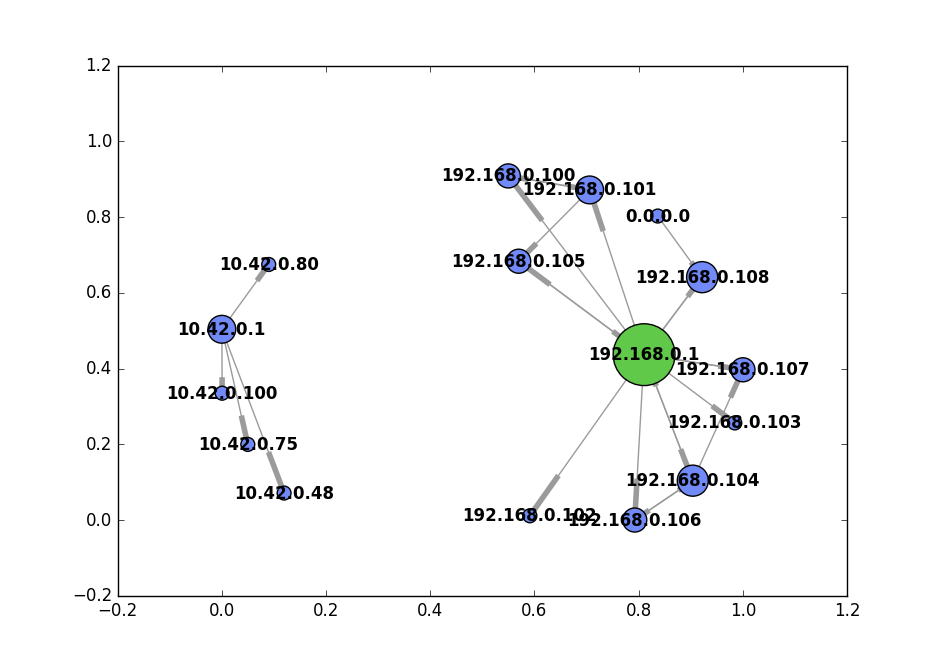
\includegraphics[width=0.8\linewidth]{imagenes/grafo-full-redLuis}
	\caption{Grafo con conexiones de nodos no distinguidos}
	\label{fig:grafo-full-redLuis}
\end{figure}

Se observan dos puntos interesantes:
 \begin{itemize}
 	\item El primero es la aparición de un nuevo conjunto de nodos que aparentemente forman una red, este tráfico corresponde a paquetes broadcast que son capturados ya que la traza fue realizada en "modo promiscuo", es decir, capturando todo el tráfico que la tarjeta de red puede "ver".
 \item El segundo es la aparición de un nodo con IP "0.0.0.0'', analizando en detalle la traza nos dimos cuenta que se trataba de un paquete broadcast ''Who-has'' enviado por un dispositivo que intentaba conectarse por primera vez a la red, al principio no posee IP, por eso está con el valor nulo "0.0.0.0", pregunta por cierta IP (192.168.0.108), que es la que intentará utilizar desde ese momento, como no está asignada se la adjudica a través de un \textit{Gratuitous ARP}, que básicamente sirve para anunciar a la red que IP está utilizando. Además este dispositivo tiene una interacción bastante frecuente con el default gateway.
 \end{itemize}
 
La entropía de la fuente es aproximadamente la mitad de la  máxima, el default gateway es el que menos información aporta, seguido por el nodo que obtiene la IP 192.168.0.108 mencionado anteriormente, el default gateway de la red externa capturada por la traza y el nodo con IP 192.168.0.104 que corresponde a una impresora. El resto de los nodos son los que aportan más información (símbolos con menor frecuencia).

\begin{figure}[H]
\centering
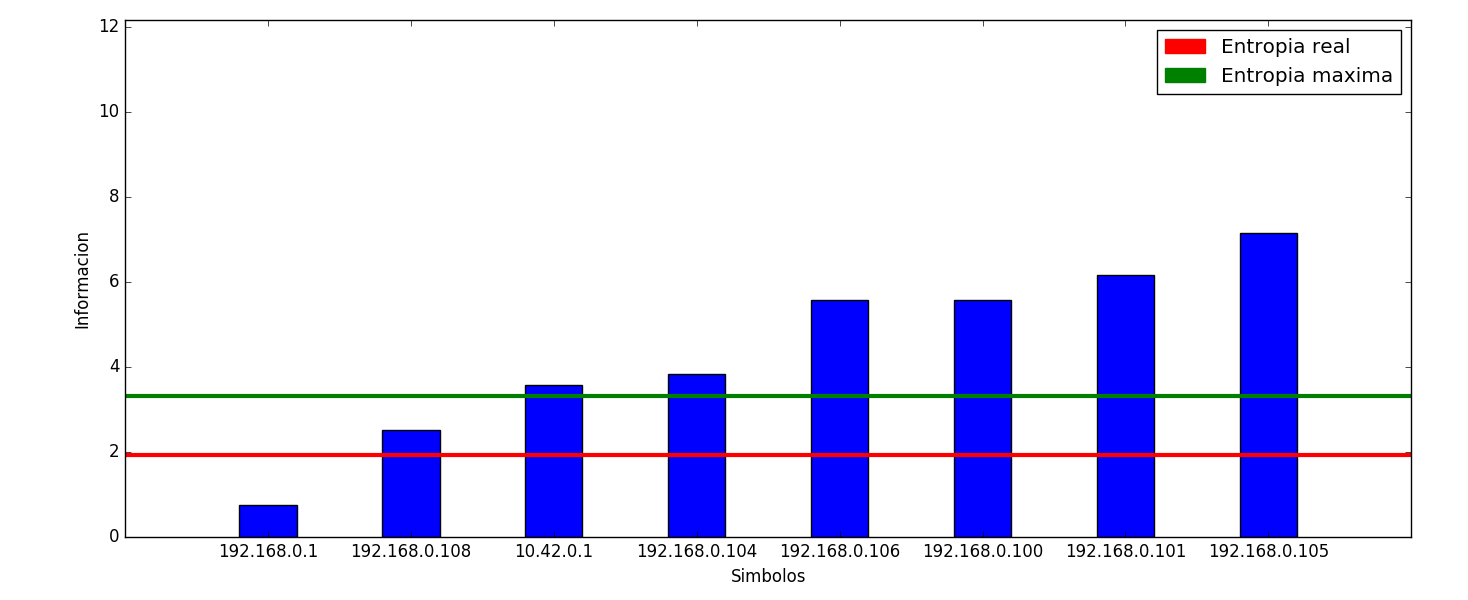
\includegraphics[width=0.8\linewidth]{imagenes/red-dom-S1}
\caption{}
\label{fig:red-dom-S1}
\end{figure}

En este caso la detección de nodos distinguidos parece ser bastante precisa para detectar default gateways, a pesar que se escucha tráfico de otras redes.